\section{Projets}
\framewithtitle{Projets}

\begin{frame}{Consignes générales}
  Ça y est, l'heure de l'évaluation est arrivée !
  Voici quelques consignes pour votre projet de fin de module.

  \begin{itemize}
    \item Je vais présenter des sujets différents, choisissez-en \textbf{un seul}.
    \item Aucun problème si un sujet n'est pas pourvu/choisi par beaucoup d'étudiants.
    \item Les instructions donnent des pistes, ne sont pas exhaustives.
    \item Développez une application qui a \textbf{du sens pour vous}.
    \item Tous les projets contiennent du Solidity et vous devrez tester vos smart contracts.
    \item Envoyez votre code source et vos tests sur GitHub.
    \item Sécurité avant tout : je serais le hacker qui tentera d'exploiter votre protocole.
    \item La pression, on la boit :)
  \end{itemize}
\end{frame}

\begin{frame}{Projet 1 : Casino avec nombres aléatoires issus de Chainlink VRF}
  Vous souhaitez construire un casino dans la blockchain.
  Pour cela, vous devrez imaginer un jeu de hasard permettant de parier de l'Ether.

  Le hasard n'existant pas dans la blockchain Ethereum, vous utiliserez le service Chainlink VRF pour générer vos nombres aléatoires.

  Règles du jeu  :

  \begin{itemize}
    \item Chaque joueur envoie la quantité d'Ether de son choix
    \item Quand tous le dernier joueur a envoyé son part, un nombre aléatoire est tiré
    \item À partir du nombre, le jeu choisi un gagnant
    \item Le gagnant rafle tout !
  \end{itemize}
\end{frame}
\begin{frame}{Projet 2 : Faucet React (front-end)}

  \begin{columns}
    \begin{column}{0.57\textwidth}
      Le but de ce projet est de créer une application web React qui aura pour but de permettre à un utilisateur de demander à recevoir des tokens ERC-20.
      Pour cette application, il faudra :

      \begin{itemize}
        \item créer un token ERC-20 de votre choix
        \item utiliser React (je suggère Next.js / Vite) et la bibliothèque Wagmi pour les smart contracts
        \item l'utilisateur appellera lui-même la fonction de mint
        \item bonus : inclure une limite de requêtes/montant par jour
      \end{itemize}
    \end{column}
    \begin{column}{0.37\textwidth}
      \resizebox{\textwidth}{!}{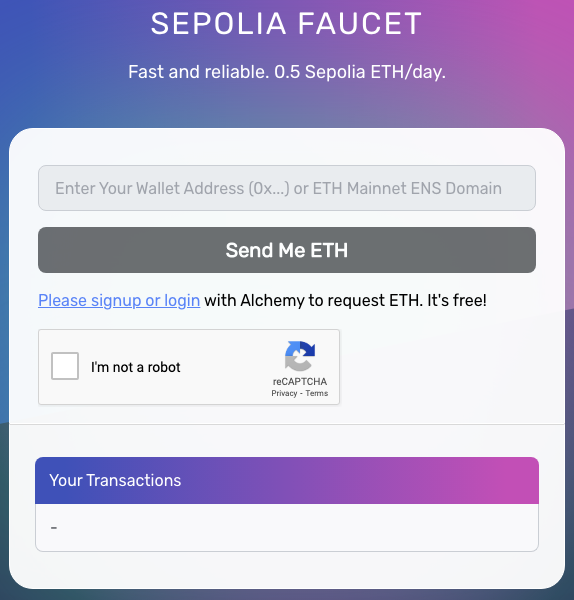
\includegraphics{img/faucet.png}}
    \end{column}
    \hspace{0.03\textwidth}
  \end{columns}
\end{frame}
\begin{frame}{Projet 3 : Marketplace NFT}
  Implémentez un marketplace NFT permettant de mettre en vente des NFT au standard ERC-721.
  Sur cet échange, il y aura deux acteurs : les vendeurs et les acheteurs.

  Les vendeurs peuvent :

  \begin{itemize}
    \item mettre en vente un NFT à un certain prix en Ether ou ERC-20
    \item changer le prix d'une de leurs offres
    \item annuler une de leurs offres
  \end{itemize}

  Les acheteurs peuvent :

  \begin{itemize}
    \item accepter une offre d'un vendeur s'il possède les tokens nécessaire
  \end{itemize}

  Le contrat doit exposer des functions permettant de lister les offres par collection (adresse du token ERC-721).
\end{frame}
\begin{frame}{Projet 4 : Système de vote par token ERC-20}
  Les organisations autonomes décentralisées (DAO) sont des acteurs majeurs des blockchains.
  Elles permettent de gouverner des projets grâce à des sytèmes de vote décentralisés.

  Vous devrez créer un token ERC-20 qui permet d'accéder à un contrat de vote.
  Ce contrat permettrat au détenteurs du tokens de voter des propositions \textbf{au prorata} de leur balance.

  Les fonctionnalités attendues sont :

  \begin{itemize}
    \item tout détenteur de plus de X tokens peut faire une proposition (à vous de choisir la structure de donnée d'une proposition...)
    \item tout vote pour toute propisition possède une date de fermeture
    \item tout détenteur de tokens peut voter pour une proposition (oui/non)
    \item \textbf{attention : assurez-vous que les tokens d'un utilisateur ne puissent pas être utilisés plusieurs fois}
    \item bonus : implémentez un quorum minimum à atteindre pour qu'un proposition soit acceptée
  \end{itemize}
\end{frame}
\begin{frame}{Projet 5 : Plateforme de Staking}
  Le staking consiste à détenir et à bloquer des tokens pour soutenir les opérations du réseau blockchain et en tirer des récompenses.
  Il permet aux détenteurs de participer à la sécurisation du réseau et de gagner des intérêts sur leurs avoirs.

  Développez un système permettant à des détenteurs d'un token ERC=20 de bloquer leurs tokens et de gagner des récompenses sur le temps.
  Les fonctionnalités attendues sont :

  \begin{itemize}
    \item tout détenteur peut bloquer tout ou une partie de ses tokens pour une durée déterminée
    \item durant cette période, l'utilisateur va obtenir des récompenses en fonction de la quantité de tokens bloqués et de la durée depuis de le début du staking
    \item à la fin de la période de stakiong, l'utilisateur peut :
          \begin{itemize}
            \item retirer ses tokens et ses récompenses
            \item re-staker ses tokens et ses récompenses
          \end{itemize}
  \end{itemize}
\end{frame}
\begin{frame}{Projet 6 : Jeu de prédiction}
  Les cryptomonnaies sont connues pour leur grande volatilité.
  Le but de ce projet est de proposer aux utilisateurs de parier sur la montée ou la descente d'actifs.

  Vous utiliserez les \href{https://docs.chain.link/data-feeds/price-feeds}{Chainlink Data Feeds} comme source de vérité pour les prix.

  Les fonctionnalités attendues sont les suivantes :

  \begin{itemize}
    \item tout utilisateur peut placer une prédiction sur une cryptomonnaie et sur la montée / descente (à vous de définir les règles exactes)
    \item les gains des gagnants sont payés par les mises des perdants
    \item le contrat doit conserver une commission d'un certain pourcentage sur les gain
  \end{itemize}
\end{frame}
\begin{frame}[fragile]{Projet 7 : Collection de NFT avec des traits}
  Les collections de NFTs possèdent bien souvent des traits, qui des caractéristiques off-chains.
  Les traits des NFT sont définis dans un fichier JSON dont l'URL est renvoyée par la fonction :

  \begin{minted}{solidity}
    interface IERC721Metadata {
      function tokenURI(uint256 tokenId) returns (string memory);
    }
  \end{minted}

  Créez une collection de NFT mintable via un contrat de vente supportant les traits :

  \begin{itemize}
    \item exposer les manifestes JSON des tokens via une petite application back-end (langage au choix)
    \item stockez les caractéristiques des tokens dans une base de données
    \item générez les traits au hasard loresqu'un token est minté :
          \begin{itemize}
            \item soit en utilisant un client Ethereum et en écoutant les events de Mint
            \item soit en utilisant le produit \href{https://www.alchemy.com/notify/custom-webhooks}{Alchemy Custom Webhooks}
          \end{itemize}
  \end{itemize}
\end{frame}